\documentclass[conference]{IEEEtran}
\IEEEoverridecommandlockouts

\usepackage{cite}
\usepackage{amsmath,amssymb}
\usepackage{graphicx}
\usepackage{booktabs}
\usepackage{xcolor}
\usepackage{url}
\usepackage{textcomp}
\usepackage{algorithm}
\usepackage{algorithmic}
\usepackage{tikz}
\usetikzlibrary{positioning,arrows.meta,calc}
\def\BibTeX{{\rm B\kern-.05em{\sc i\kern-.025em b}\kern-.08em T\kern-.1em\lower.7ex\hbox{E}\kern-.125em X}}

% Numbers below are generated from benchmark_results.json / grace_results.json (make_tables.py)
\newcommand{\domPrec}{100.0}
\newcommand{\domRec}{100.0}
\newcommand{\domFone}{1.000}
\newcommand{\domFound}{311}
\newcommand{\domSpur}{0}
\newcommand{\domRoom}{100.0}
\newcommand{\domRoomN}{311}
\newcommand{\domPass}{19}
\newcommand{\domTotalSec}{15.4}
\newcommand{\ocrPrec}{57.1}
\newcommand{\ocrRec}{53.1}
\newcommand{\ocrFone}{0.550}
\newcommand{\ocrFound}{165}
\newcommand{\ocrSpur}{124}
\newcommand{\ocrRoom}{39.5}
\newcommand{\ocrRoomN}{123}
\newcommand{\ocrPass}{2}
\newcommand{\ocrTotalSec}{32.1}
\newcommand{\nCases}{19}
\newcommand{\nSlots}{311}
\newcommand{\nStd}{12}
\newcommand{\nAdv}{7}
\newcommand{\SZeroFourOcrFound}{21}
\newcommand{\SZeroFourTruth}{60}
\newcommand{\SZeroFourOcrSpur}{31}
\newcommand{\SZeroFourOcrSec}{6.4}
\newcommand{\SZeroFourDomSec}{1.9}
\newcommand{\AZeroFiveOcrFound}{29}
\newcommand{\AZeroFiveTruth}{60}
\newcommand{\AZeroFiveOcrSpur}{30}
\newcommand{\AZeroFiveOcrSec}{6.3}
\newcommand{\AZeroFiveDomSec}{1.9}
\newcommand{\SZeroFiveOcrFound}{1}
\newcommand{\SZeroFiveTruth}{10}
\newcommand{\SZeroFiveOcrSpur}{5}
\newcommand{\SZeroFiveOcrSec}{1.0}
\newcommand{\SZeroFiveDomSec}{0.6}
\newcommand{\SZeroTwoOcrFound}{26}
\newcommand{\SZeroTwoTruth}{30}
\newcommand{\SZeroTwoOcrSpur}{11}
\newcommand{\SZeroTwoOcrSec}{3.6}
\newcommand{\SZeroTwoDomSec}{1.3}
\newcommand{\speedup}{3.4}
\newcommand{\GOnePZeroZeroFrag}{0.0}
\newcommand{\GOnePZeroZeroMae}{0.00}
\newcommand{\GOnePZeroZeroSess}{1.000}
\newcommand{\GOnePZeroOneFrag}{12.3}
\newcommand{\GOnePZeroOneMae}{1.37}
\newcommand{\GOnePZeroOneSess}{1.131}
\newcommand{\GOnePZeroTwoFrag}{22.8}
\newcommand{\GOnePZeroTwoMae}{2.70}
\newcommand{\GOnePZeroTwoSess}{1.257}
\newcommand{\GOnePZeroFiveFrag}{45.8}
\newcommand{\GOnePZeroFiveMae}{6.48}
\newcommand{\GOnePZeroFiveSess}{1.607}
\newcommand{\GOnePOneZeroFrag}{69.7}
\newcommand{\GOnePOneZeroMae}{12.81}
\newcommand{\GOnePOneZeroSess}{2.166}
\newcommand{\GTwoPZeroZeroFrag}{0.0}
\newcommand{\GTwoPZeroZeroMae}{0.00}
\newcommand{\GTwoPZeroZeroSess}{1.000}
\newcommand{\GTwoPZeroOneFrag}{0.1}
\newcommand{\GTwoPZeroOneMae}{0.07}
\newcommand{\GTwoPZeroOneSess}{1.002}
\newcommand{\GTwoPZeroTwoFrag}{0.5}
\newcommand{\GTwoPZeroTwoMae}{0.18}
\newcommand{\GTwoPZeroTwoSess}{1.004}
\newcommand{\GTwoPZeroFiveFrag}{3.0}
\newcommand{\GTwoPZeroFiveMae}{0.70}
\newcommand{\GTwoPZeroFiveSess}{1.030}
\newcommand{\GTwoPOneZeroFrag}{10.3}
\newcommand{\GTwoPOneZeroMae}{2.26}
\newcommand{\GTwoPOneZeroSess}{1.108}
\newcommand{\GThreePZeroZeroFrag}{0.0}
\newcommand{\GThreePZeroZeroMae}{0.00}
\newcommand{\GThreePZeroZeroSess}{1.000}
\newcommand{\GThreePZeroOneFrag}{0.0}
\newcommand{\GThreePZeroOneMae}{0.05}
\newcommand{\GThreePZeroOneSess}{1.000}
\newcommand{\GThreePZeroTwoFrag}{0.0}
\newcommand{\GThreePZeroTwoMae}{0.10}
\newcommand{\GThreePZeroTwoSess}{1.000}
\newcommand{\GThreePZeroFiveFrag}{0.2}
\newcommand{\GThreePZeroFiveMae}{0.29}
\newcommand{\GThreePZeroFiveSess}{1.002}
\newcommand{\GThreePOneZeroFrag}{1.1}
\newcommand{\GThreePOneZeroMae}{0.78}
\newcommand{\GThreePOneZeroSess}{1.011}
\newcommand{\simTrials}{300}


\begin{document}

\title{DOM-Based Participant Attendance Tracking for Google Meet Breakout Rooms:\\
A Comparison with OCR-Based Screen Reading}

\author{\IEEEauthorblockN{Harsha Sunkavalli}
\IEEEauthorblockA{\textit{Department of Computer Science}\\
\textit{George Mason University}\\
smasriharsha@gmail.com}}

\maketitle

\begin{abstract}
Taking attendance in video meetings that use breakout rooms is tedious to do by hand, and the official reporting available to a host does not always fit the need. An earlier tool addressed this by taking screenshots of the Google Meet participant panel and recovering names with optical character recognition (OCR). That design is exposed to every property of the rendered pixels: fonts, scripts, zoom, layout and overlays. This paper presents a replacement that reads participant names and breakout-room membership directly from the page's Document Object Model (DOM) through browser automation, and feeds them to a session engine that tolerates transient read errors with a grace period and back-dated leave times. We compare the two methods by running the \emph{real} implementation of each on identical mock Meet-style panels in headless Chromium, over \nCases{} test cases (\nStd{} standard, \nAdv{} adversarial) containing \nSlots{} participant slots. The DOM tracker recovered \domFound{} of \nSlots{} names exactly (\domRec\%), produced \domSpur{} spurious names, and placed \domRoom\% of names in the correct room. The OCR tracker recovered \ocrFound{} (\ocrRec\%), produced \ocrSpur{} spurious names, and placed \ocrRoom\% correctly. On a 60-person list the DOM scan was \speedup$\times$ faster. A seeded simulation shows that a two-scan grace period reduces split attendance records from \GOnePZeroFiveFrag\% to \GTwoPZeroFiveFrag\% at a 5\% per-scan read-miss rate. The evaluation uses mock pages, not a live Meet call, and the OCR implementation was tuned on real screens, so its scores here likely understate its field accuracy; we discuss these limits and give a first-run procedure for validating the DOM selectors on live meetings.
\end{abstract}

\begin{IEEEkeywords}
attendance tracking, Google Meet, breakout rooms, DOM extraction, optical character recognition, browser automation, web data extraction
\end{IEEEkeywords}

%--------------------------------------------------------------------
\section{Introduction}
Online meetings with breakout rooms are common in teaching, training and community organizations, and organizers often need to know who attended, in which room, and for how long. Doing this by hand during a session is slow and error-prone, particularly when a participant list has dozens of entries and people move between the main call and several rooms. The original motivation for this work was a volunteer organization that held weekly Google Meet sessions with breakout rooms; its tool, written by the author, replaced manual head counts with timestamped CSV reports and, as reported by the author, saved several hours of administrative work per session. That figure is anecdotal and is not measured in this paper.

The original tool is \emph{vision based}. It opens the breakout-rooms panel under browser automation, takes screenshots while scrolling, finds the panel's left edge by pixel colour analysis, runs Tesseract OCR \cite{smith2007tesseract} over three image variants, groups recognized words into lines, infers room headers from text patterns, splits side-by-side name chips by horizontal gaps, filters recognition noise with regular expressions, and detects presence dots with colour masks in OpenCV \cite{bradski2000opencv}. This works, but each stage encodes assumptions about appearance. Names that contain accents, non-Latin scripts or emoji are hard for the recognizer; a different zoom, theme or layout can move the panel edge; and a mid-scan layout change must be detected and discarded. Errors are \emph{silent}: the output is a plausible but wrong name.

The page that is being photographed already contains the answer in structured form. The participant list is part of the DOM \cite{whatwg2024dom}, and Meet, like other web applications, exposes much of its UI through accessibility attributes defined by WAI-ARIA \cite{w3c2023aria}. This paper asks whether reading that structure instead of the pixels yields a more accurate, faster and more maintainable attendance tracker, and what new risks it introduces.

\textbf{Contributions.}
\begin{enumerate}
\item A DOM-based tracker design for Meet attendance, including breakout-room assignment from document order, scroll-and-merge for virtualized lists, and a layered architecture in which only one component touches the browser.
\item A session engine with a grace period and back-dated leave times, and a fail-safe rule that an empty read is never treated as ``everyone left''.
\item A head-to-head evaluation that runs the real implementations of both methods on identical pages: \nCases{} cases, \nSlots{} participant slots, reported with precision, recall, F1, room accuracy and scan time, plus a seeded simulation of the grace-period trade-off.
\item An account of defects found by the verification process itself, and an explicit statement of what the evaluation does \emph{not} establish.
\end{enumerate}
The source code, benchmark harness, raw results and this paper are in the project repository \cite{repo}.

The remainder of the paper is organized as follows. Section~\ref{sec:related} reviews background. Section~\ref{sec:problem} formalizes the task. Sections~\ref{sec:ocr} and~\ref{sec:dom} describe the baseline and the proposed system. Section~\ref{sec:method} gives the experimental method, Section~\ref{sec:results} the results, and Section~\ref{sec:discussion} discusses limits and ethics. Section~\ref{sec:conclusion} concludes.

%--------------------------------------------------------------------
\section{Background and Related Work}\label{sec:related}
\subsection{Attendance in Google Meet}
Meet's participant panel lists who is in the call and, for a host using breakout rooms, which room each person is in \cite{meethelp}. Official programmatic interfaces and administrator reports exist for some account types; their availability and the data they expose depend on the account and edition. This work follows the original tool's constraint of needing no API access, using only the signed-in host's browser, and we did not evaluate official interfaces.

\subsection{OCR and screen reading}
OCR converts images of text into character sequences and has a long history \cite{mori1992historical}. Tesseract \cite{smith2007tesseract} is a widely used open-source engine. Accuracy depends on resolution, contrast, font and script, and the output is a best guess with a confidence score rather than a ground-truth string. Using OCR on a rendered user interface inherits these limits and adds layout analysis: deciding which recognized words form one name, which are decoration, and which belong to which section.

\subsection{Web data extraction and the DOM}
Web data extraction is the problem of recovering structured data from web pages; surveys distinguish approaches that rely on page structure from those that rely on rendered appearance \cite{ferrara2014web}. Structure-based extraction is attractive when markup is stable, but brittle when it is not. Browser automation interfaces such as WebDriver \cite{w3c2018webdriver} (implemented by Selenium \cite{selenium}) and Playwright \cite{playwright} let a program evaluate JavaScript inside the page and return values. WAI-ARIA \cite{w3c2023aria} defines roles (\texttt{list}, \texttt{listitem}, \texttt{heading}) and properties (\texttt{aria-label}, \texttt{aria-expanded}) that exist for assistive technology and are therefore more stable than the generated CSS class names typical of large web applications. Our selector strategy is built on that observation.

\subsection{Evaluation measures}
We use precision, recall and F1 \cite{manning2008ir,powers2011evaluation}, defined in Section~\ref{sec:method}. Fuzzy string similarity, used only to count near-miss recognitions, is based on the Ratcliff--Obershelp gestalt matching algorithm \cite{ratcliff1988gestalt}.

%--------------------------------------------------------------------
\section{Problem Formulation}\label{sec:problem}
Let a meeting be observed at scan times $t_1<\dots<t_K$ separated by an interval $\Delta$ (300\,s in real use). At scan $k$ the visible panel yields a snapshot
\begin{equation}
S_k=\{(r,n)\}, \quad r\in\mathcal{R},\; n\in\mathcal{N},
\end{equation}
a set of (room, display-name) pairs, where the main call is a room. A tracker is a pair $(\mathcal{E},\mathcal{A})$: an \emph{extractor} $\mathcal{E}$ that maps the page to a snapshot $\hat S_k$, and an \emph{attendance engine} $\mathcal{A}$ that maps the snapshot sequence to sessions $(r,n,t_{\text{join}},t_{\text{leave}})$. The report is the set of sessions.

We want an extractor that (i) recovers names exactly, so that reports can be matched to rosters; (ii) assigns each name to the right room; (iii) emits few or no spurious names; (iv) fails visibly; and (v) is cheap to run and to maintain. We want an engine whose sessions are not fragmented by isolated read errors and whose durations are accurate to within roughly one scan interval. The tracker's own account is excluded from the report.

%--------------------------------------------------------------------
\section{Baseline: OCR Pipeline}\label{sec:ocr}
The baseline extractor $\mathcal{E}_{\text{OCR}}$ proceeds as follows for each scroll position of the panel:
\begin{enumerate}
\item Capture a screenshot and detect the panel's left edge by scanning columns for the dark panel background, then crop.
\item Upscale by two and run Tesseract on three variants (contrast-adjusted, inverted, and CLAHE-enhanced), merging words that fall in the same position bucket.
\item Group words into lines by vertical position; derive room headers from text (``Main call'', ``Breakout $N$ Join'', lines containing ``room'').
\item Assign each remaining line to the nearest header above it; split lines into names where horizontal gaps are large; remove strings that match noise phrases, fragments, or lowercase-initial text.
\item For each name, crop a region of interest and test for a green or yellow circular blob in HSV space as a presence cue.
\item Merge scroll positions, treating the first screenshot's room list as canonical so that rooms first seen after scrolling are ignored, and discard the whole scan if screenshot widths differ by more than 100\,px (layout change).
\end{enumerate}
The method embodies many tuned constants and text patterns. Its strengths are that it needs no knowledge of page internals and that it observes what a human would see.

%--------------------------------------------------------------------
\section{Proposed System: DOM-Based Tracker}\label{sec:dom}
\subsection{Architecture}
Fig.~\ref{fig:arch} shows the layers. Only the \emph{Panel reader} interacts with the browser. Everything after it is plain Python, which makes the engine, normalization and report writer testable without a browser. A scan loop runs in its own thread and a stop event ends it and flushes reports.

\begin{figure*}[t]
\centering
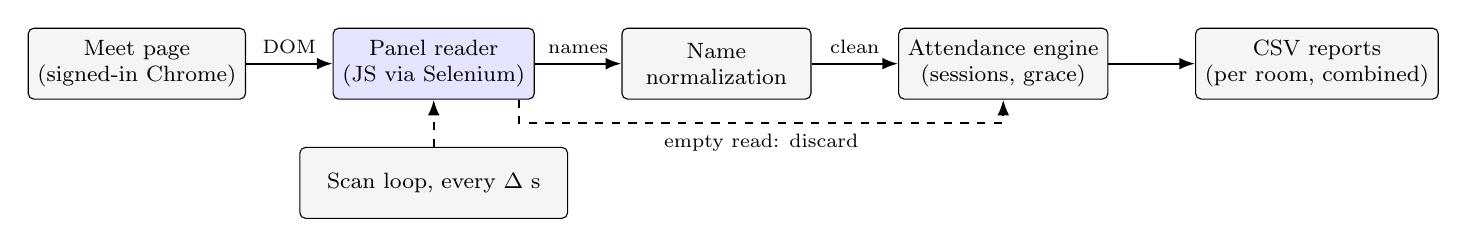
\begin{tikzpicture}[
  node distance=7mm and 11mm,
  box/.style={draw, rounded corners=2pt, minimum height=9mm, minimum width=24mm, align=center, font=\footnotesize, fill=gray!8},
  hot/.style={box, fill=blue!10},
  arr/.style={-{Latex[length=2mm]}, thick}]
  \node[box] (meet) {Meet page\\(signed-in Chrome)};
  \node[hot, right=of meet] (reader) {Panel reader\\(JS via Selenium)};
  \node[box, right=of reader] (norm) {Name\\normalization};
  \node[box, right=of norm] (eng) {Attendance engine\\(sessions, grace)};
  \node[box, right=of eng] (rep) {CSV reports\\(per room, combined)};
  \draw[arr] (meet) -- node[above,font=\scriptsize]{DOM} (reader);
  \draw[arr] (reader) -- node[above,font=\scriptsize]{names} (norm);
  \draw[arr] (norm) -- node[above,font=\scriptsize]{clean} (eng);
  \draw[arr] (eng) -- (rep);
  \node[box, below=6mm of reader, minimum width=34mm] (loop) {Scan loop, every $\Delta$ s};
  \draw[arr, dashed] (loop) -- (reader);
  \draw[arr, dashed] (reader.south east) ++(-2mm,0) -- ++(0,-3mm) -| node[pos=0.25,below,font=\scriptsize]{empty read: discard} ($(eng.south)+(0,-0mm)$);
\end{tikzpicture}
\caption{DOM tracker architecture. The shaded component is the only one that touches the browser; the engine discards empty reads so a failed scan never ends sessions.}
\label{fig:arch}
\end{figure*}

\subsection{Locating and scrolling the panel}
The reader finds visible \texttt{role="list"} elements that contain list items, walks up to the nearest scrollable ancestor, and scrolls it from top to bottom in steps of 80\% of its height, extracting at each step and de-duplicating by (room, raw name). This handles \emph{virtualized} lists, which keep only visible rows in the DOM. A bounded number of steps guards against runaway loops. If the panel is closed the reader tries to open it from the toolbar by accessible label.

\subsection{Structural extraction}
Algorithm~\ref{alg:extract} gives the extraction walk, executed in the page. It relies on document order: a heading-like element starts a new room section, and every list item belongs to the current section.

\begin{algorithm}[t]
\caption{Room-aware extraction (runs in the page)}\label{alg:extract}
\begin{algorithmic}[1]
\STATE $room \leftarrow$ \textsc{MainCall};\ $out \leftarrow [\,]$
\FOR{each element $e$ under the panel, in document order}
  \IF{$e$ has role \texttt{listitem}}
    \STATE $name \leftarrow$ first non-empty of: data attribute, \texttt{aria-label}, nested \texttt{aria-label}, first text line
    \STATE append $(room, name)$ to $out$
  \ELSIF{$e$ is not inside a \texttt{listitem} and is a heading, \texttt{h2}/\texttt{h3}, or has \texttt{aria-expanded}}
    \STATE $txt \leftarrow$ first line of $e$ without trailing ``$(N)$'' and ``Join''
    \IF{$txt\neq\emptyset$, $|txt|<60$, and $txt\notin$ \textsc{NotRoom}}
      \STATE $room \leftarrow$ \textsc{MainCall} if $txt$ matches ``main call''; else $txt$
    \ENDIF
  \ENDIF
\ENDFOR
\RETURN $out$
\end{algorithmic}
\end{algorithm}

Two design choices matter. First, room names are not matched against a naming pattern: any heading outside a participant row that is not a known section title (``People'', ``Contributors'', ``Breakout rooms'', and similar) is a room, so custom names work. Second, headings inside a participant row are ignored, because rows commonly contain buttons with \texttt{aria-expanded} (for example a ``more actions'' menu) that would otherwise be misread as rooms. The first rule replaced an earlier pattern-based version that failed on headings such as ``Breakout 1'' (Section~\ref{sec:defects}).

\subsection{Name normalization}
Raw strings from the DOM are normalized before use: zero-width characters are removed, whitespace is collapsed, trailing decorations such as ``(You)'', ``(Host)'' and ``(Presentation)'' are stripped (repeatedly), and full Meet phrases such as ``Pin $X$ to your main screen'' and ``More actions for $X$'' are unwrapped. Strings that are UI words (``Mute'', ``Host'', ``Contributors'') or contain no letters are rejected. Names are keyed case- and whitespace-insensitively. Only \emph{full phrases} are unwrapped, not bare verbs, so a participant named ``Pin Sharma'' is preserved.

\subsection{Attendance engine}
Algorithm~\ref{alg:engine} summarizes the update rule. A participant is considered to have left only after $g$ consecutive scans without them (default $g=2$), and the recorded leave time is back-dated to the last scan at which they were seen. At shutdown, anyone who was already missing is closed at their last-seen time rather than at the stop time; all others are closed at the stop time.

\begin{algorithm}[t]
\caption{Engine update for one room and scan at time $t$}\label{alg:engine}
\begin{algorithmic}[1]
\STATE $V \leftarrow \{\textsc{key}(n) : n\in \text{normalized names}, n\ne\text{self}\}$
\FOR{$v\in V$}
  \STATE $miss[v]\leftarrow 0$;\ $last[v]\leftarrow t$
  \IF{$v\notin present$} \STATE open session $(v, t_{\text{join}}{=}t)$; add $v$ to $present$ \ENDIF
\ENDFOR
\FOR{$v\in present\setminus V$}
  \STATE $miss[v]\leftarrow miss[v]+1$
  \IF{$miss[v]\ge g$} \STATE close session with $t_{\text{leave}}\leftarrow last[v]$; remove $v$ \ENDIF
\ENDFOR
\end{algorithmic}
\end{algorithm}

\subsection{Failure handling and diagnostics}
If the panel is closed and cannot be reopened, or the extraction returns nothing (for example because selectors went stale), the scan is skipped and the engine receives no update. This prevents a failure from being recorded as everyone leaving. A diagnostic mode captures the panel's HTML and the parsed result for a live meeting, so that selectors can be adjusted when Meet's markup changes. All Meet-specific selectors are isolated in a small set of JavaScript constants.

\subsection{Implementation}
The tracker is a single Python file of 484 lines (versus 1{,}072 for the OCR tool) depending on Selenium, undetected-chromedriver and pandas; it needs no image-processing library and no OCR binary. It writes the same CSV schema as the baseline (room, name, join time, leave time, duration in minutes, date), one combined file and one per room.

%--------------------------------------------------------------------
\section{Experimental Method}\label{sec:method}
\subsection{Mock-panel harness}
A live Meet call could not be used for this study, so each test case is a mock panel that imitates Meet's side panel (dark theme, rows with avatar and name, section headings) rendered in headless Chromium at $1366\times768$. For each case the \emph{same page} is given to both trackers: the DOM tracker's real \texttt{PanelReader} runs its JavaScript in the page through an adapter that mimics the Selenium script-execution interface, and the OCR tracker's real code (screenshot cropping, panel-edge detection, Tesseract 5.3.4, cleaning and merge) processes screenshots of the same page taken at each scroll position. Both outputs are compared with known ground truth. Nothing in either implementation was replaced by a stub apart from the browser-launch dependency of the OCR module.

\subsection{Test cases}
Table~\ref{tab:cases} lists the \nCases{} cases. The \nStd{} standard cases vary size (5, 30 and 60 people), the number of rooms, name difficulty (accents, Chinese, Cyrillic, emoji, apostrophes, hyphens, lowercase), the markup style (\texttt{h2} headings, \texttt{aria-expanded} headings, rows without \texttt{aria-label}, nested \texttt{aria-label}), empty rooms, and a chip layout in the style the OCR code was written for (S11, S12). The \nAdv{} adversarial cases target the DOM method specifically: decorated labels with the tracker's own row (A01), per-row action buttons with \texttt{aria-expanded} (A02), non-room section titles (A03), custom and non-English room names (A04), a virtualized 60-row list (A05), one person listed twice (A06) and a closed panel (A07).

\subsection{Metrics}
Names are compared case- and whitespace-insensitively. Let $T$ be the set of true names, $G$ the set output, and $D=T\cap G$. \emph{Recall} $=|D|/|T|$; \emph{precision} $=|D|/|G|$; $F_1$ is their harmonic mean; \emph{room accuracy} is the fraction of $T$ that were reported in the correct room (rooms are compared after canonicalization, so ``Main call'' equals ``Main Call'' and ``Breakout 1'' equals ``Breakout Room 1''). \emph{Spurious} names are $G\setminus T$. A case \emph{passes} only if recall, precision and room accuracy are all 100\%. Aggregate figures pool all slots; A07 has no participants and contributes only to spurious counts and pass/fail.

\subsection{Grace-period simulation}
To study the engine in isolation we simulate 50 participants over a 90-minute meeting with scans every 5 minutes (19 scans). Half stay throughout and half leave permanently at a random scan. At each scan every present participant is independently missed with probability $p\in\{0,1,2,5,10\}\%$, modelling transient read errors. For $g\in\{1,2,3\}$ we run \simTrials{} meetings per cell with fixed seeds, using the real engine, and record the fraction of participants whose attendance is split into more than one session and the mean absolute error of total recorded minutes against truth.

\subsection{Unit tests}
Twenty-five offline tests cover name normalization (Unicode, emoji, decorations, noise words, wrapped phrases), the engine (grace values, rejoin, room moves, self exclusion, duplicates, shutdown back-dating, 100-person roster, concurrent access), the CSV schema, and the failed-scan safety rule.

%--------------------------------------------------------------------
\section{Results}\label{sec:results}
\subsection{Aggregate accuracy}
Table~\ref{tab:aggregate} gives the pooled results. The DOM tracker passed all \domPass{} cases; the OCR tracker passed \ocrPass{}. DOM recovered every name exactly and placed every name in the correct room with no spurious output. OCR recovered \ocrFound{} of \nSlots{} names, output \ocrSpur{} names that were not real, and placed \ocrRoomN{} names in the correct room.

\begin{table}[t]
\caption{Aggregate accuracy over 19 cases and 311 participant slots}
\label{tab:aggregate}
\centering\footnotesize
\begin{tabular}{lrr}
\toprule
Metric & DOM & OCR \\
\midrule
Cases passed (all names, no extras, right rooms) & 19/19 & 2/19 \\
Recall (\%) & 100.0 & 53.1 \\
Precision (\%) & 100.0 & 57.1 \\
F1 (pooled) & 1.000 & 0.550 \\
Room accuracy (\%) & 100.0 & 39.5 \\
Spurious names output & 0 & 124 \\
Total scan time, all cases (s) & 15.4 & 32.1 \\
\bottomrule
\end{tabular}
\end{table}


\subsection{Per-case results}
Fig.~\ref{fig:cases} and Table~\ref{tab:cases} show the cases. OCR was accurate on the smallest baseline (S01) and on the most benign adversarial cases but degraded with list length, name difficulty and markup variation. On the 60-person lists it recovered \SZeroFourOcrFound{} of \SZeroFourTruth{} (S04) and \AZeroFiveOcrFound{} of \AZeroFiveTruth{} (A05) names and output \SZeroFourOcrSpur{} and \AZeroFiveOcrSpur{} spurious names. On the hard-name case (S05) it recovered \SZeroFiveOcrFound{} of \SZeroFiveTruth{}. On the chip layout built to resemble its own conventions (S11, S12) and on the duplicated-row case (A06) it recovered none; on inspection, its S11 output consisted of last-name fragments such as ``Brown'' and ``Wilson''.

\begin{figure*}[t]
\centering
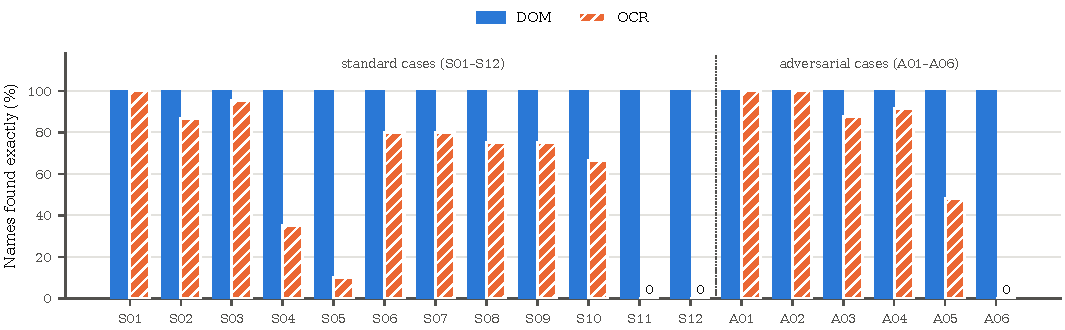
\includegraphics[width=\textwidth]{figures/per_case_recall.pdf}
\caption{Names recovered exactly per case (A07 omitted: no participants). A label ``0'' marks a case where OCR recovered no name exactly.}
\label{fig:cases}
\end{figure*}

\begin{table*}[t]
\caption{Per-case results. \emph{Found} = real names recovered exactly; \emph{Extra} = output names that are not real; \emph{Room} = names in the correct room. $n$ = real participants.}
\label{tab:cases}
\centering\footnotesize
\begin{tabular}{llrcrrcrrrr}
\toprule
 & & & \multicolumn{2}{c}{DOM} & & \multicolumn{4}{c}{OCR} & \\
\cmidrule(lr){4-5}\cmidrule(lr){7-10}
ID & Description & $n$ & Found & Extra & & Found & Extra & Room & Time (s) \\
\midrule
S01 & Baseline, 5 people, 1 room & 5 & 5 & 0 & & 5 & 0 & 5 & 0.8 \\
S02 & 30 people, Main Call & 30 & 30 & 0 & & 26 & 11 & 26 & 3.6 \\
S03 & Main + 3 breakout rooms & 22 & 22 & 0 & & 21 & 3 & 3 & 2.4 \\
S04 & 60 people, 3 rooms, scrolled & 60 & 60 & 0 & & 21 & 31 & 15 & 6.4 \\
S05 & Accents, CJK, Cyrillic, emoji & 10 & 10 & 0 & & 1 & 5 & 1 & 1.0 \\
S06 & Headings as \texttt{<h2>} & 10 & 10 & 0 & & 8 & 3 & 4 & 1.0 \\
S07 & Headings via \texttt{aria-expanded} & 10 & 10 & 0 & & 8 & 3 & 4 & 1.1 \\
S08 & Rows without \texttt{aria-label} & 8 & 8 & 0 & & 6 & 3 & 6 & 0.9 \\
S09 & Nested \texttt{aria-label} & 8 & 8 & 0 & & 6 & 3 & 6 & 0.9 \\
S10 & Empty rooms between rooms & 6 & 6 & 0 & & 4 & 3 & 2 & 0.9 \\
S11 & OCR-native chip layout & 18 & 18 & 0 & & 0 & 6 & 0 & 0.7 \\
S12 & OCR-native chips, 30 people & 30 & 30 & 0 & & 0 & 13 & 0 & 1.4 \\
\midrule
A01 & Decorated labels + own row & 6 & 6 & 0 & & 6 & 1 & 6 & 0.8 \\
A02 & Per-row action buttons & 6 & 6 & 0 & & 6 & 0 & 6 & 0.7 \\
A03 & Non-room section titles & 8 & 8 & 0 & & 7 & 3 & 7 & 1.0 \\
A04 & Custom/non-English room names & 12 & 12 & 0 & & 11 & 5 & 3 & 1.2 \\
A05 & Virtualized list, 60 people & 60 & 60 & 0 & & 29 & 30 & 29 & 6.3 \\
A06 & One person listed twice & 2 & 2 & 0 & & 0 & 0 & 0 & 0.6 \\
A07 & Panel not open & 0 & 0 & 0 & & 0 & 1 & 0 & 0.6 \\
\bottomrule
\end{tabular}
\end{table*}


\subsection{Scan time}
Fig.~\ref{fig:time} plots the time for one full scan against list size. The DOM scan is dominated by fixed waits between scroll steps (about 0.6\,s) and grows slowly with list length; OCR time grows with the number of screenshots and recognition passes. At 60 participants, DOM took \SZeroFourDomSec{}\,s and OCR \SZeroFourOcrSec{}\,s, a ratio of \speedup$\times$. Over all cases the totals were \domTotalSec{}\,s and \ocrTotalSec{}\,s. These are single-run timings on one machine and are indicative only.

\begin{figure}[t]
\centering
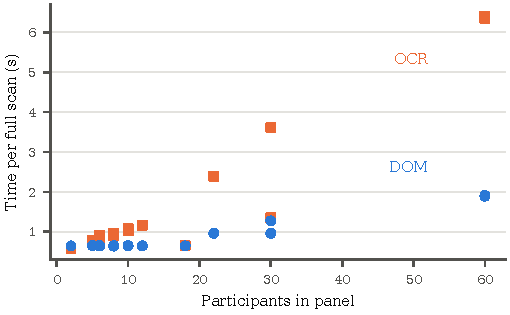
\includegraphics[width=\columnwidth]{figures/scan_time.pdf}
\caption{Time for one full scan versus participants in the panel, one point per case.}
\label{fig:time}
\end{figure}

\subsection{Effect of the grace period}
Fig.~\ref{fig:grace} and Table~\ref{tab:grace} show the simulation. With $g=1$ (leave on the first missed scan) split attendance is already \GOnePZeroOneFrag\% at a 1\% miss rate and reaches \GOnePZeroFiveFrag\% at 5\%, with a mean duration error of \GOnePZeroFiveMae{} minutes. With $g=2$ the same 5\% miss rate gives \GTwoPZeroFiveFrag\% split attendance and \GTwoPZeroFiveMae{} minutes of error; with $g=3$ it gives \GThreePZeroFiveFrag\% and \GThreePZeroFiveMae{} minutes. Because leave times are back-dated to the last observation, a larger grace period does not inflate durations; its cost is that a real departure is reported by the live log $g$ scans later, and that tracking of someone who rejoins within the window is continuous rather than split. Without read errors ($p=0$) all settings are exact.

\begin{figure}[t]
\centering
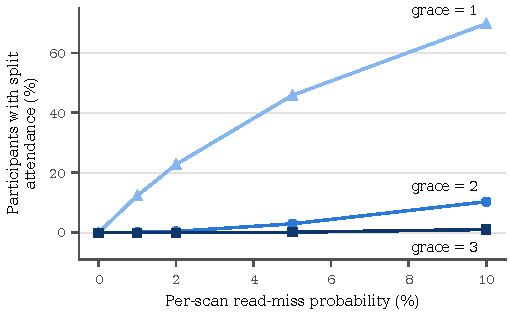
\includegraphics[width=\columnwidth]{figures/grace_fragmentation.pdf}
\caption{Participants whose attendance was split into several sessions versus the per-scan read-miss probability, for grace periods of 1, 2 and 3 scans.}
\label{fig:grace}
\end{figure}

\begin{table}[t]
\caption{Grace-period simulation (300 meetings per cell, 50 participants, 19 scans). Cells: participants with split attendance (\%) / mean absolute duration error (min).}
\label{tab:grace}
\centering\footnotesize
\begin{tabular}{lccc}
\toprule
Miss prob. & grace=1 & grace=2 & grace=3 \\
\midrule
0\% & 0.0 / 0.00 & 0.0 / 0.00 & 0.0 / 0.00 \\
1\% & 12.3 / 1.37 & 0.1 / 0.07 & 0.0 / 0.05 \\
2\% & 22.8 / 2.70 & 0.5 / 0.18 & 0.0 / 0.10 \\
5\% & 45.8 / 6.48 & 3.0 / 0.70 & 0.2 / 0.29 \\
10\% & 69.7 / 12.81 & 10.3 / 2.26 & 1.1 / 0.78 \\
\bottomrule
\end{tabular}
\end{table}


\subsection{Defects found by verification}\label{sec:defects}
Running the harness exposed three defects in the DOM tracker, each now fixed and covered by a unit test.
\begin{enumerate}
\item \emph{Room-heading detection was too narrow.} The first version recognized only headings of the form ``Breakout Room \dots'' and filed participants under ``Breakout 1'' or ``Group A'' in the main call. Detection now accepts any heading-like element outside a participant row that is not a known section title.
\item \emph{Name unwrapping stripped bare verbs.} A leading ``Pin'' or ``Mute'' was removed from names, turning ``Pin Sharma'' into ``Sharma''. Only full Meet phrases are unwrapped now.
\item \emph{Shutdown over-credited departures.} The simulation showed non-zero duration error even without read errors when $g>1$: at shutdown, a person who had already left but was still inside the grace window was credited up to the stop time. Leave times for such participants are now back-dated to their last observation.
\end{enumerate}
The first two were found by test cases and the third by the simulation, which is an argument for testing the session logic separately from extraction.

%--------------------------------------------------------------------
\section{Discussion}\label{sec:discussion}
\subsection{Why the DOM approach performs better here}
Reading text from the DOM removes the recognition step, so names survive exactly, including scripts and symbols that an OCR engine tuned for Latin text handles poorly. It removes layout analysis, so room assignment follows the document structure and custom names work. It removes dependence on pixels, so zoom, theme and window size do not matter. It also changes the failure mode: a stale selector yields an empty read that is detected and skipped, whereas an OCR error yields a wrong name that looks valid.

\subsection{What OCR still offers}
OCR needs no knowledge of the page's internals and therefore survives markup changes that would break DOM selectors. It also works on any application whose content can be screenshotted, where DOM access is impossible. A practical system could use the DOM method as the primary reader and fall back to OCR when selectors return nothing; we did not build or evaluate such a hybrid.

\subsection{Threats to validity}
\textbf{Mock pages.} The most important limit is that the pages are mocks. They follow Meet's accessibility structure as understood by the author, but the real markup may differ, particularly in how breakout-room headings and rows are exposed. The 100\% DOM result shows that the extraction logic is robust across many plausible markups; it does not show that the tracker works on Meet today. The provided diagnostic mode and a first-run checklist are intended to close that gap.

\textbf{OCR is likely understated.} The OCR implementation was tuned on real Meet screens, and the mock only approximates real fonts, chips and colours. Its absolute scores here, notably the zero on the chip layout, are therefore best read as sensitivity to layout rather than as production accuracy.

\textbf{OCR language model.} The original tool does not select a Tesseract language, so recognition used the default English model. The very low score on the hard-name case (S05) partly reflects this; installing additional language models might improve non-Latin names, and we did not test that.

\textbf{Tuning on the benchmark.} The DOM extractor was corrected after the first benchmark run exposed a defect, so its final result is partly tuned to these cases. A fresh set of live pages is the real test.

\textbf{Construct and scope.} Exact name matching counts a one-character recognition error as a miss. The simulation assumes independent read errors, whereas real errors are likely correlated in time (for example during a re-render). Only one run per case on one machine was made. Two different participants with an identical display name cannot be told apart by either tracker, and neither case was evaluated.

\subsection{Privacy, consent and platform terms}
Attendance data are personal data. Organizers should tell participants that attendance is recorded and handle the CSV files accordingly. The tool automates a signed-in browser session and uses a driver intended to avoid bot detection; users should check that this is consistent with the platform's terms for their account type and prefer sanctioned interfaces where those meet their needs. The source code stores no credentials; login is manual.

%--------------------------------------------------------------------
\section{Conclusion and Future Work}\label{sec:conclusion}
We replaced a vision-based Meet attendance tracker with one that reads participant names and room membership from the DOM and tracks sessions with a grace period. On identical mock panels, the DOM tracker recovered all \nSlots{} names with no spurious output and correct rooms in all \nCases{} cases, while the OCR tracker recovered \ocrRec\% of names and \ocrRoom\% of room assignments, and the DOM scan was several times faster on long lists. A simulation showed that a two-scan grace period removes most fragmentation caused by transient read errors, and the verification process itself uncovered three defects that were fixed.

The principal next step is validation on live meetings using the provided diagnostic mode. Further work includes using stable participant identifiers if the page exposes them, so that identical display names can be separated; replacing polling with a \texttt{MutationObserver} for event-driven join and leave times; a hybrid DOM-primary, OCR-fallback reader; a comparison with official reporting interfaces where available; and a study over many real sessions with a hand-verified roster.

%--------------------------------------------------------------------
\section*{Reproducibility}
All code, the harness (\texttt{verify\_dom\_vs\_ocr.py}), the simulation (\texttt{paper/grace\_simulation.py}), the raw results (\texttt{benchmark\_results.json}, \texttt{paper/grace\_results.json}) and the scripts that generate this paper's tables and figures are in the repository \cite{repo}. The accuracy, timing and simulation numbers in the text and tables are generated from those result files; other figures (such as source line counts) are stated directly.

\bibliographystyle{IEEEtran}
\bibliography{references}

\end{document}
